\documentclass{article}
\usepackage[utf8]{inputenc}
\usepackage{amsmath}
\usepackage[linesnumbered,ruled]{algorithm2e}
\usepackage{mathtools}
\usepackage{commath}
\usepackage{bm}
\usepackage{hyperref}
\usepackage{tikz}
\usepackage{placeins}
\usetikzlibrary{shapes.geometric, arrows}

\title{Xenobot technical report \\  Lane following}
\author{\textbf{Shengwen Cheng , Po-Sheng Chen}}
\date{January 2017}

\begin{document}

\maketitle

\tikzstyle{blocks} = [rectangle, rounded corners, minimum width=2cm, minimum height=1cm,text centered, draw=black, fill=orange!30]
\tikzstyle{arrow} = [thick,->,>=stealth]

\section{Introduction}
Xenobot is a computer vision based self-driving system inspired by MIT duckietown project. We re-implement our own system for real-time robotics research and may add more new features in the future.
\\
The algorithm we're using is a modified version of MIT duckietown, so you can find many similarities between two projects. This report is focus on how our lane following algorithm works.
\\
\\
\\
\\

\begin{figure}[ht]
  \label{fig:xenobot}
  \centering
  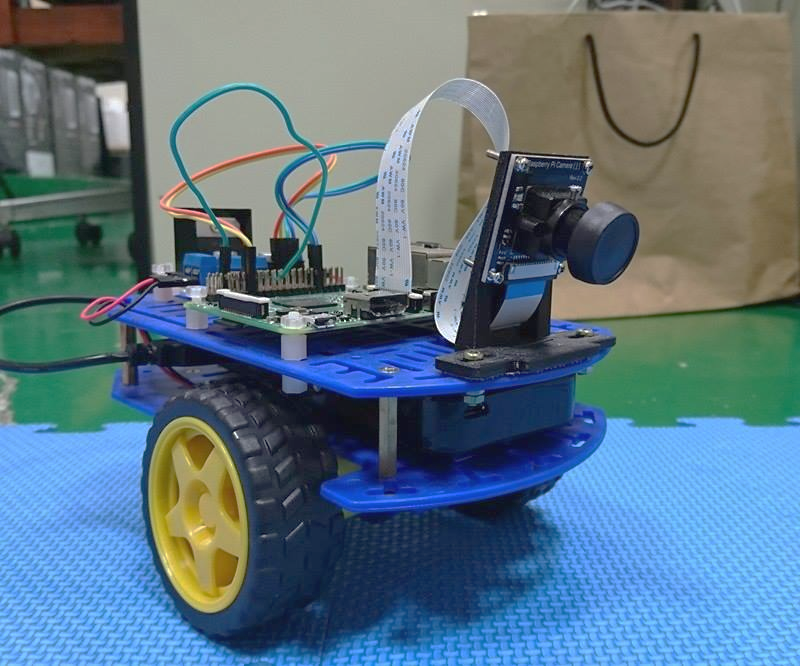
\includegraphics[scale=0.3]{graphs/xenobot.PNG}
  \caption{Xenobot}
\end{figure}

\clearpage

\section{Camera calibrations}

Camera calibration is a big issue for computer vision. The camera parameter tells us the mapping between the image and the real world.

\subsection{Intrinsic parameters}

Intrinsic parameter describe the mapping between 2D image frame and 3D camera frame, usually also dealing with the distortion or skew of the camera.

\subsection{Extrinsic parameters}

Extrinsic parameters describe the rotation and translation of the camera with respect to the world frame.

\clearpage

\section{Lane pose estimation}

\subsection{Lane pose and system conventions}
\begin{figure}[ht]
  \label{fig:lane_coordination}
  \centering
  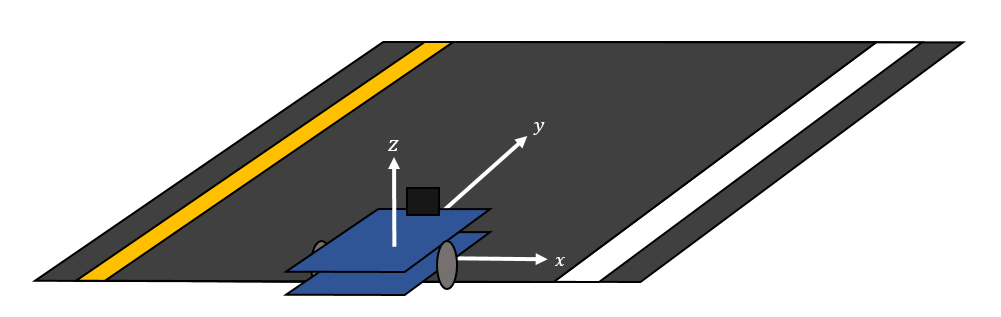
\includegraphics[scale=0.6]{graphs/coordinate_system.PNG}
  \caption{Lane coordination}
\end{figure}
\FloatBarrier

\begin{figure}[ht]
  \label{fig:lane_2d_view}
  \centering
  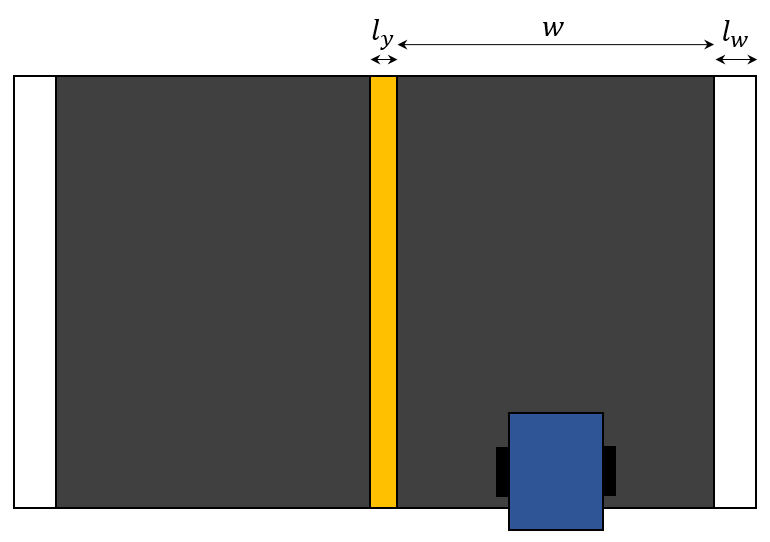
\includegraphics[scale=0.6]{graphs/lane_parameter_2d_view.PNG}
  \caption{2D view of lane}
\end{figure}
\FloatBarrier

\begin{figure}[ht]
  \label{fig:lane_pose}
  \centering
  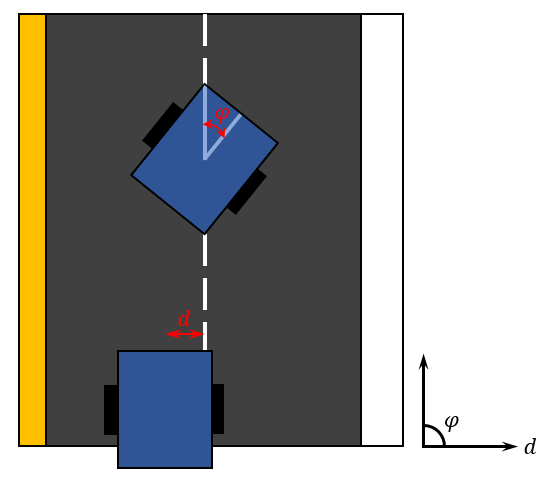
\includegraphics[scale=0.7]{graphs/lane_pose.PNG}
  \caption{Lane pose}
\end{figure}
\FloatBarrier

\subsection{Segements detection}

The first step for lane pose estimation is to extract the segments from the image, the process to do this is to threshold the specific color we want, and apply canny edge detector and Hough transform so we can find out the location of those segments

\begin{figure} [ht]
\begin{center}
\begin{tikzpicture}[node distance=2cm]
\node (raw) [blocks, yshift=0cm] {Raw image} ;
\node (rectify) [blocks, yshift=-1.5cm] {Distortion and rectification};
\node (canny) [blocks, xshift=-2cm, yshift=-3cm] {Canny edge detection};
\node (diliation_canny) [blocks, xshift=-2cm, yshift=-4.5cm] {Diliation};
\node (threshold) [blocks, xshift=2cm, yshift=-3cm] {HSV color thresholding};
\node (diliation_threshold) [blocks, xshift=2cm, yshift=-4.5cm] {Diliation};
\node (and) [blocks, yshift=-6cm] {Bitwise And};
\node (hough) [blocks, yshift=-7.5cm] {Hough transform};
\node (segments) [blocks, yshift=-9cm] {Segments};

\draw [arrow] (raw) -- (rectify);
\draw [arrow] (rectify) -- (canny);
\draw [arrow] (canny) -- (diliation_canny);
\draw [arrow] (rectify) -- (threshold);
\draw [arrow] (threshold) -- (diliation_threshold);
\draw [arrow] (diliation_canny) -- (and);
\draw [arrow] (diliation_threshold) -- (and);
\draw [arrow] (and) -- (hough);
\draw [arrow] (hough) -- (segments);
\end{tikzpicture}
\end{center}
\caption{Work flow of lane detector}
\end{figure}
\FloatBarrier


\subsection{Frame transformation}

The segments we got in the lane detector stage is in the camera frame, however, what we are really interested is the car frame, so we need to do a transformation between these two frame.

\[
\begin{pmatrix} x_{car} \\ y_{car} \end{pmatrix} = 
\begin{pmatrix} x_{camera} - r \cdot \sin\phi \\ y_{camera} - r \cdot \cos\phi \end{pmatrix}
\]

\begin{figure}[ht]
  \label{fig:frame_transformation}
  \centering
  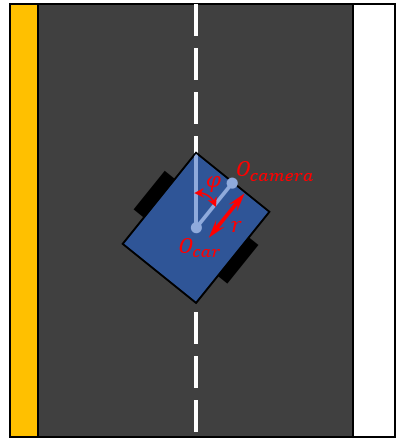
\includegraphics[scale=0.7]{graphs/frame_transformation.PNG}
  \caption{Frame transformation}
\end{figure}
\FloatBarrier

\subsection{Segment side recognition}
We obtained the lane segments during the lane detection process. Next step is to figure out the segment side on the lane mark. It could be determined by reading multiple pixel values in the direction of segment normal vector on color thresholding image.

\begin{figure}[ht]
  \label{fig:lane_segment}
  \centering
  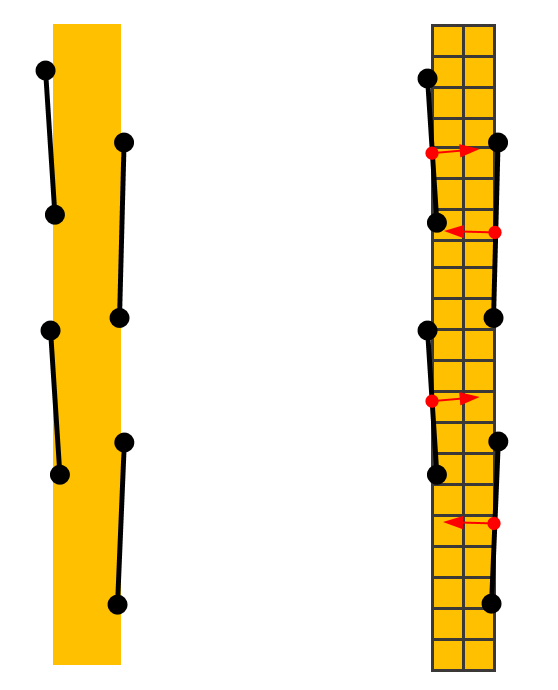
\includegraphics[scale=0.4]{graphs/segment.PNG}
  \caption{Lane segments}
\end{figure}
\FloatBarrier

\begin{figure} [ht]
\begin{algorithm}[H]
	\KwData{segment, accumulator threshold, color binarization image}
	\KwResult{side (left or right)}
	$\vec{P_1} = (x_1, y_1)$
	\\
	$\vec{P_2} = (x_2, y_2)$
	\\
	$\vec{P} = (\vec{P_1} + \vec{P_2}) / 2$
	\\
	$\vec{t} = \frac{\vec{P_2} - \vec{P_1}}
					{\norm{\vec{P_2} - \vec{P_1}}}$
	\\
	$\vec{n} = (-y_t, x_t)$
	\\
	\For {$i < pixel \ count$} {
		$x \gets \lceil x_p + x_n \cdot i \rceil$
		\\
		$y \gets \lceil y_p + y_n \cdot i \rceil$
		\\		
		\uIf{$I(x,y) = I_{max}$}
			{
				$left \gets left + 1$ 
			}
			
		$x \gets \lfloor x_p - x_n \cdot i \rfloor$
		\\
		$y \gets \lfloor y_p - y_n \cdot i \rfloor$
		\\		
		\uIf{$I(x,y) = I_{max}$}
			{
				$right \gets right + 1$ 
			}
	}
	
	\uIf {$left > threshold \ \& \  right < threshold$}
		{
			\Return is left
		}
	\uElseIf {$right > threshold \ \& \ left < threshold$}
		{
			\Return is right
		}
	\uElse
		{
			\Return unknown side
		} 
	\caption{Segment side recognition}
\end{algorithm}
\end{figure}
\FloatBarrier

\subsection{Segment pose estimation}

\begin{figure}[ht]
  \label{fig:lane_geometry}
  \centering
  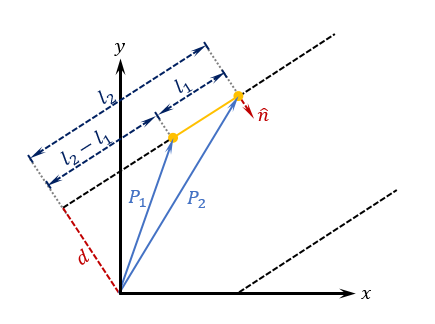
\includegraphics[scale=1]{graphs/lane_geometry.PNG}
  \caption{Lane geometry}
\end{figure}
\FloatBarrier

\begin{figure} [ht]
\begin{algorithm}[H]
	\KwData{segment}
	\KwResult{pose $d_{i}$ and $\phi_{i}$}
	$\vec{P_1} = (x_1, y_1)$

	$\vec{P_2} = (x_2, y_2)$

	$\vec{t} = \frac{\vec{P_2} - \vec{P_1}}
					{\norm{\vec{P_2} - \vec{P_1}}}$

	$\vec{n} = (-y_t, x_t)$

	$\phi_{i} = \arctan(\frac{y_t}{x_t}) - \pi / 2$

	\uIf {segment color = white}
		{
			\eIf{edge side = right}
			{
				$\vec{k} = (\frac{w}{2} + l_w) \cdot \vec{n}$
			}
			{
				$\vec{k} = (\frac{w}{2}) \cdot \vec{n}$
			}
		}
	\uElseIf {segment color = yellow}
		{
			\eIf{edge side = left}
			{
				$\vec{k} = (-\frac{w}{2} - l_y) \cdot \vec{n}$
			}
			{
				$\vec{k} = (-\frac{w}{2}) \cdot \vec{n}$
			}
		}
	$\vec{j} = (r \cdot \sin\phi, r \cdot \cos\phi)$

	$\vec{P_1^\prime} = \vec{P_1} + \vec{k} - \vec{j}$

	$\vec{P_2^\prime} = \vec{P_2} + \vec{k} - \vec{j}$

	$d_1 = \vec{P_1} \cdot \vec{n}$

	$d_2 = \vec{P_2} \cdot \vec{n}$

	$d_{i} = (d_1 + d_2) / 2$
	\caption{Generate vote}
\end{algorithm}
\caption{Vote generation}
\end{figure}
\FloatBarrier

\subsection{Histogram filter}

\begin{figure}[ht]
  \label{fig:histogram_filter}
  \centering
  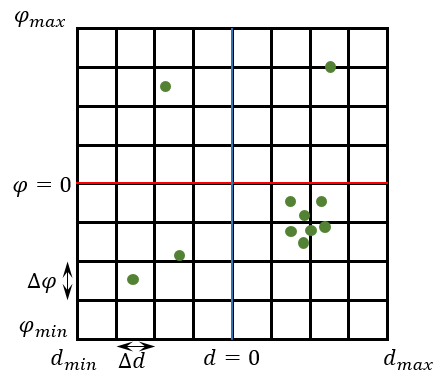
\includegraphics[scale=0.9]{graphs/histogram_filter.PNG}
  \caption{Histogram filter}
\end{figure}
\FloatBarrier

\begin{figure} [ht]
\begin{algorithm}[H]
	\KwData{segment}
	\KwResult{filtered pose $d$ and $\phi$}
	\For {$\bm{all}$ segments} {
			$(\phi_i, d_i) \gets generate\_vote(segment)$
			
			$I \gets round(\frac{\phi_i - \phi_{min}}{\Delta\phi})$

			$J \gets round(\frac{d_i - d_{min}}{\Delta d})$
			
			$histogram(I, J) \mathrel{+}= 1$
	}
	
	$(I_{highest}, J_{highest}) \gets find \_ highest \_ vote()$	
	
	$\phi_{histogram} \gets I_{highest} \cdot \Delta \phi + \phi_{min}$
	
	$d_{histogram} \gets J_{highest} \cdot \Delta d + d_{min}$

	$\phi_{mean} \gets 0 \ , \  d_{mean} \gets 0$
	
	$N_{\phi} \gets 0 \ , \ N_{d} \gets 0$
	
	\For {$\bm{all} \ (\phi_{i}, d_{i})$}
	{
		\uIf {$\phi_{i} \in [\phi_{histogram} - \frac{\Delta \phi}{2}, 
			  \phi_{histogram} + \frac{\Delta \phi}{2}]$}
		{
			$\phi_{mean} \mathrel{+}= \phi_{i}$
			
			$N_{\phi} \mathrel{+}= 1$
		}
		
		\uIf {$d_{i} \in [d_{histogram} - \frac{\Delta d}{2}, 
			  d_{histogram} + \frac{\Delta d}{2}]$}
		{
			$d_{mean} \mathrel{+}= d_{i}$
			
			$N_{d} \mathrel{+}= 1$
		}
	}
	
	$\phi_{mean} \gets \frac{\phi_{mean}}{N_{\phi}}$
	
	$d_{mean} \gets \frac{d_{mean}}{N_{d}}$	
	\caption{Histogram filter}
\end{algorithm}
\caption{Histogram filter}
\end{figure}
\FloatBarrier

\clearpage

\section{Control system}

\subsection{Differential wheels}

\subsection{PID Controller}
The equation of PID controller in continuous time is given as:\\

\[e(t) = setpoint(t) - x(t)\]

\[u(t) = K_p e(t) + K_i \int_{0}^{t} e(\tau) d\tau + K_d  \frac{de(t)}{dt}\]

in discreted time:

\[e[t] = setpoint[t] - x[t]\]

\[u(t) = K_p e[t] + K_i \sum_0^t e[t] \Delta t + K_d \frac{e[t] - e[t-1]}{\Delta t}\]

\subsection{d control and phi control}

The lane pose controller of Xenobot is a cascaded PID controller, the phi controller is treat as a low level contoller for lane orientation stablizing, the higher level d controller will change the setpoint of the phi controller to turn left or right back to the middle of road when it is needed.

\begin{figure}[ht]
  \label{fig:control_diagram}
  \centering
  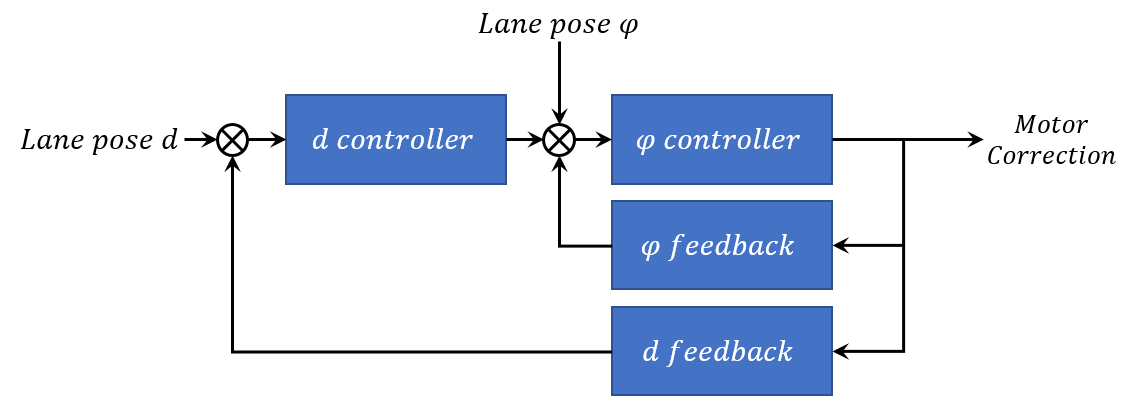
\includegraphics[scale=0.6]{graphs/control_diagram.PNG}
  \caption{Control diagram}
\end{figure}
\FloatBarrier

\clearpage

\section{References}

[1] Lane Filter by Liam Paull, MIT CSAIL

\end{document}